\documentclass[letterpaper,11pt]{article}

\usepackage{latexsym}
\usepackage[empty]{fullpage}
\usepackage{titlesec}
\usepackage{marvosym}
\usepackage[usenames,dvipsnames]{color}
\usepackage{verbatim}
\usepackage{enumitem}
\usepackage[hidelinks]{hyperref}
\usepackage{fancyhdr}
\usepackage[UTF8]{ctex}
\usepackage{multirow}
\usepackage{graphicx}
\usepackage{tabularx}
\usepackage{eso-pic}
\usepackage{svg}

\pagestyle{fancy}
\fancyhf{} % clear all header and footer fields
\fancyfoot{}
\renewcommand{\headrulewidth}{0pt}
\renewcommand{\footrulewidth}{0pt}

% Adjust margins
\addtolength{\oddsidemargin}{-0.375in}
\addtolength{\evensidemargin}{-0.375in}
\addtolength{\textwidth}{1in}
\addtolength{\topmargin}{-.5in}
\addtolength{\textheight}{1.0in}

\urlstyle{same}

\raggedbottom
\raggedright
\setlength{\tabcolsep}{0in}

% Sections formatting
\titleformat{\section}{
  \vspace{-4pt}\scshape\raggedright\large
}{}{0em}{}[\color{black}\titlerule \vspace{-5pt}]

%-------------------------
% Custom commands
\newcommand{\resumeItem}[2]{
  \item\small{
    \textbf{#1}{ #2 \vspace{-2pt}}
  }
}

\newcommand{\resumeSubheading}[4]{
  \vspace{-1pt}\item
    \begin{tabular*}{0.97\textwidth}{l@{\extracolsep{\fill}}r}
      \textbf{#1} & #2 \\
      \textit{\small#3} & \textit{ #4} \\
    \end{tabular*}\vspace{-5pt}
}

\newcommand{\resumeSubheadingtwo}[2]{
  \vspace{-1pt}\item
    \begin{tabular*}{0.97\textwidth}{l@{\extracolsep{\fill}}r}
      \textbf{#1} & \textit{ #2} \\
      % \textit{\small#3} & \textit{\small #4} \\
    \end{tabular*}\vspace{-5pt}
}

\newcommand{\resumeSubItem}[2]{\resumeItem{#1}{#2}\vspace{-4pt}}

\renewcommand{\labelitemii}{$\circ$}

\newcommand{\resumeSubHeadingListStart}{\begin{itemize}[leftmargin=*]}
\newcommand{\resumeSubHeadingListEnd}{\end{itemize}}
\newcommand{\resumeItemListStart}{\vspace{-10pt}\begin{itemize}}
\newcommand{\resumeItemListEnd}{\end{itemize}\vspace{-10pt}}

\newcommand{\basicInfo}[1]{
  \centerline{\sffamily\large{#1}}
  \vspace{1.5ex}
}

\newcommand{\name}[1]{
  \centerline{\Large\songti{#1}}
  \vspace{1.25ex}
}

%-------------------------------------------
%%%%%%  CV STARTS HERE  %%%%%%%%%%%%%%%%%%%%%%%%%%%%


\begin{document}

%----------HEADING-----------------

% \name{赵子琦}
% \basicInfo{
%   \href{mailto:zziqi@buaa.edu.cn}{zziqi@buaa.edu.cn} \textperiodcentered\ 
%   \href{tel:+8617813063387}{ 178-1306-3387}    \textperiodcentered\ 
%   zzq229cr}

\begin{minipage}[t]{0.12\textwidth}
  % \vspace*{-2.5cm} % 调整垂直位置
  % 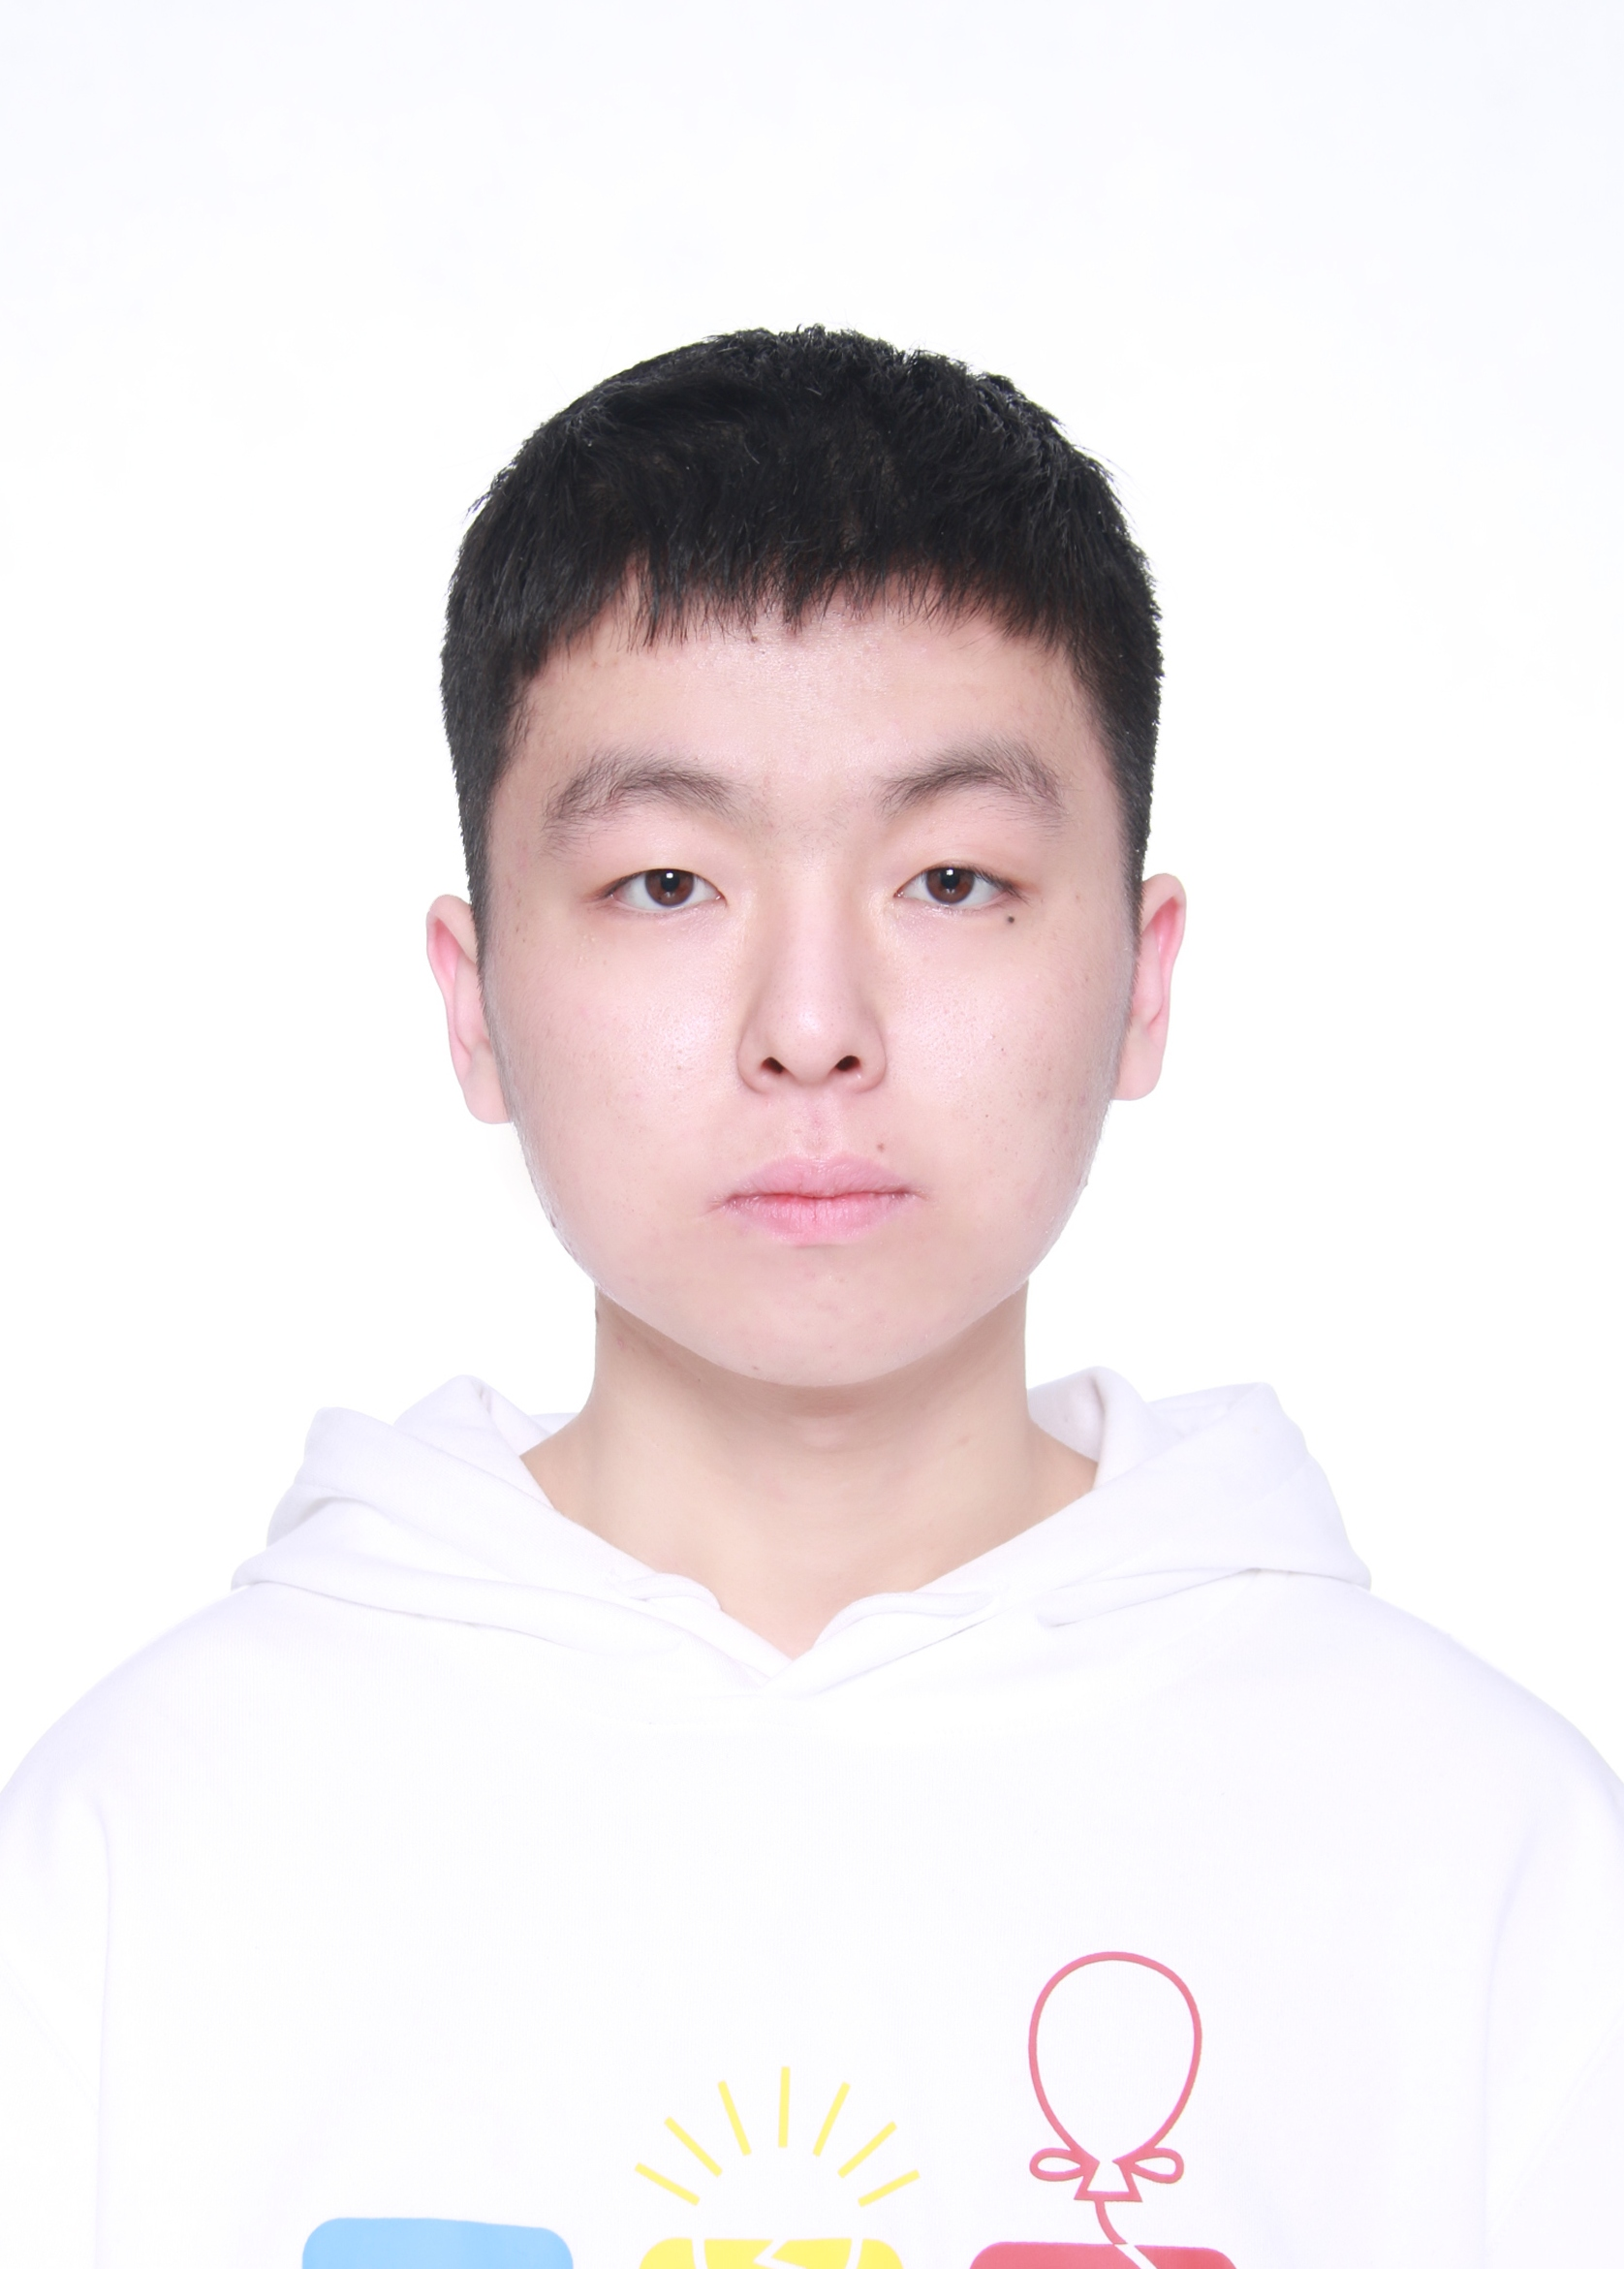
\includegraphics[width=\textwidth]{zzqpic.jpg}
\end{minipage}
\hfill
\begin{minipage}[t]{0.7\textwidth}
      \name{\textbf{赵子琦}}
      \basicInfo{
        \href{mailto:zziqi229@gmail.com}{ \raisebox{-0.2\height}{
\includegraphics[width=12pt]{envelope.pdf}} zziqi229@gmail.com} \textperiodcentered\ 
        \href{tel:17813063387}{ \raisebox{-0.18\height}{
\includegraphics[width=11pt]{phone.pdf}} 178-1306-3387}    \textperiodcentered\ 
        \raisebox{-0.2\height}{
\includegraphics[width=13pt]{weixin.pdf}} zzq229cr}
\end{minipage}%
\hfill
\begin{minipage}[t]{0.12\textwidth}
    \vspace*{-1cm} % 调整垂直位置
    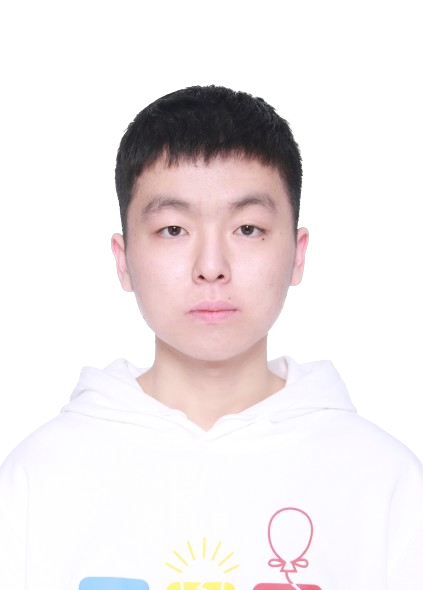
\includegraphics[width=\textwidth]{zzqpic-no-bg.png}
\end{minipage}


%-----------EDUCATION-----------------
\vspace{-29pt}
\section{教育经历}
  \resumeSubHeadingListStart
    \resumeSubheading
      {北京航空航天大学}{北京}
      {计算机科学与技术;  硕士在读, 2025年毕业}{2022年9月 -- 至今}
    \resumeSubheading
      {哈尔滨工程大学}{哈尔滨, 黑龙江}
      {计算机科学与技术;  排名: 4/315, 前1.3\%}{2018年9月 -- 2022年6月}
  \resumeSubHeadingListEnd

\vspace{-10pt}
\section{实习经历}
    \begin{itemize}[leftmargin=*,itemsep=-10pt]
        \resumeSubheadingtwo
            {字节跳动 Data-AML-科学计算}{2023年5月 -- 至今}
            \\[10pt]
            % \resumeItem{开发}
            弹性算力平台开发和维护,屏蔽业务场景和资源平台的复杂性,为各类业务提供简洁、一致的使用接口.\\
            独立负责一部分核心功能开发,做出性能和稳定性优化优化,提升平台稳定性和任务通量.
            \vspace*{0.8em}
            \resumeItemListStart
                 \resumeItem{}
                {基于 k8s 调度器设计开发 ai4s-scheduler 调度器组件,基于潮汐和不稳定资源实现混合调度和优先级调度,为业务提供更灵活的调度策略.}
                \resumeItem{}
                {设计开发任务调度,提高任务调度效率和稳定性,支持FIFO调度和机房亲和性调度,支持任务失败快速重试.}
                \resumeItem{}
                {平台性能和稳定性优化,随着平台逐渐承担更多业务和任务,定位解决各类性能瓶颈和稳定性问题.}
                \resumeItem{}
                {新特性支持,支持容器热更新、支持训练任务、SDK开发、监控告警、端到端测试等需求.}
                \resumeItem{}
                {日常Oncall支持与平台日常维护,为上层各种业务提供支持,监控线上状况及时作出针对性修复和维护.}
            \resumeItemListEnd
    \end{itemize}

\vspace{-10pt}
\section{项目经历}
    \begin{itemize}[leftmargin=*,itemsep=5pt]
        \resumeSubheadingtwo
            {MIT6.824分布式系统}{\href{https://github.com/zzq229-creator/6.824}{https://github.com/zzq229-creator/6.824}}
            % 麻省理工学院研究生课程,通过 paper reading/lectures/labs 学习和理解分布式系统的基础知识.涉及到 MapReduce、GFS、Raft、ZooKeeper、Memcached 等分布式系统领域经典论文.实验中实现MapReduce、Raft算法.
            \\[10pt]
                % {麻省理工学院研究生课程,涉及到MapReduce、GFS、Raft、ZooKeeper、Spanner、Spark等技术.并构建了一个高并发高可用的线性一致分片键值数据库.}
            \resumeItemListStart
                % \resumeItem{MapReduce}
                    % {根据MapReduce论文实现了一个分布式MapReduce框架,实现worker失效处理}
                \resumeItem{Raft算法}
                    {完整实现 Raft 算法,包括领导选举、日志复制、快照、持久化.}
                \resumeItem{键值数据库}
                    {基于Raft共识构建高可用的分片键值数据库,支持不停机扩缩数据节点、分片动态迁移、过期分片回收、配置热更新,能容忍网络丢包、网络分区、节点失效等错误下实现线性一致性.
                        % \begin{itemize}
                        %     \item 构建高可用的分布式分片配置管理器,支持增删数据节点。
                        %     \item 每个分片服务集群询问配置管理器负责一组分片,实现了分片迁移、垃圾分片回收、配置更改期间提供服务,并保证严格线性一致.
                        % \end{itemize}
                    }
            \resumeItemListEnd

        % \resumeSubheadingtwo
            % {校内信息平台}{}{}
            % {\href{https://qinglianjie.cn/}{https://qinglianjie.cn}}
            % \\[7pt]
            % 校园内网信息一站式获取,使用微服务架构和 Celery 分布式任务队列系统。拥有 5000+ 用户,提供所有课程信息查询,课表、成绩、学分查询汇总,课程出分提醒,统计课程成绩分布,实现课程论坛. 
    \end{itemize}

\vspace{-10pt}
\section{曾获奖项}
    \begin{itemize}[leftmargin=*,itemsep=-20pt]
        \resumeSubheadingtwo
          {2018-2019年度国家奖学金}{2018-2019年}
        \resumeSubheadingtwo
          {2019-2020年度校长奖学金}{2019-2020年}
      % \resumeSubItem{第 45 届 ACM/ICPC 国际大学生程序设计竞赛亚洲区域赛(上海站) 金牌}
        \resumeSubheadingtwo
          {第 45 届 ACM/ICPC 国际大学生程序设计竞赛亚洲区域赛\,金牌}{2020年12月}
        % \resumeSubheadingtwo
          % {第 44 届 ACM/ICPC 国际大学生程序设计竞赛亚洲区域赛(上海站) 银牌}{2019年11月}
        % \resumeSubheadingtwo
          % {第六届 CCPC 中国大学生程序设计竞赛(绵阳站)银牌}{2020年11月}
        \resumeSubheadingtwo
          {第五届 CCPC 中国大学生程序设计竞赛\,银牌}{2019年9月}
        \resumeSubheadingtwo
          {2020 CCF 中国大学生系统与程序设计竞赛全国总决赛\,金牌 (排名:28/1041)}{2020年10月}
        \resumeSubheadingtwo
          {2020 黑龙江省大学生程序设计竞赛\,亚军}{2020年9月}
        \resumeSubheadingtwo
          {2020 东北地区大学生程序设计竞赛\,一等奖(第4名)}{2020年10月}
        % \resumeSubheadingtwo
          % {2019 东北地区大学生程序设计竞赛 \, 一等奖}{2019年5月}
        % \resumeSubheadingtwo
          % {2019 全国大学生数学建模竞赛黑龙江赛区\,一等奖}{2019年9月}
        % \resumeSubheadingtwo
          % {第十届蓝桥杯全国软件和信息技术专业人才大赛黑龙江赛区 \, 一等奖(第4名)}{2019年3月}
    \end{itemize}


\vspace{-10pt}
\section{学术经历}
    \begin{itemize}[leftmargin=*,itemsep=-20pt]
        \resumeSubheadingtwo
            {知识图谱增强多兴趣学习的多行为推荐}{\href{https://dl.acm.org/doi/full/10.1145/3606369}{https://dl.acm.org/doi/full/10.1145/3606369},TOIS(CCF A)}
            \\[5pt]
            共同一作,首次在多行为推荐中引入多兴趣学习,挖掘用户与物品交互背后的兴趣,提出使用知识图谱提取兴趣的初始表示,结合了动态路由方案进一步探索每个行为背后的兴趣,在多个数据集上达到了最佳的推荐效果.
            % 首次在多行为推荐中引入多兴趣学习.在大多数推荐场景中存在多种行为类型(例如点击、加入购物车、购买等),不同的行为类型可能反映用户的不同兴趣。我们提出使用知识图谱提取物品的每个兴趣的初始表示,之后结合了动态路由方案进一步探索每个行为背后的兴趣。我们的模型在四个数据集上达到了最佳的推荐性能.
    \end{itemize}

\vspace{-10pt}
\section{个人}
 \resumeSubHeadingListStart
   \item{
     {热爱code \& debug,具有扎实的代码能力、优秀的算法和数据结构基础,对深度学习有一些了解.}
      % {求知欲强,有比较好的优秀的学习和沟通能力}
     % \hfill
     % \textbf{Technologies}{: AWS, Play, React, Kafka, GCE}
   }
   \item{
    求知欲强,有较好的学习和沟通能力.
   }   
   % \item{
    % 能够使用Numpy、Pandas等库进行数据处理、分析
   % }
 \resumeSubHeadingListEnd


%-------------------------------------------
\end{document}
